%------------------------------------------------------------------------------
\section{Modelo de Información: Proceso de gestión de tareas}

\subsection{Descripción General}
En la figura \ref{fig:MOD02} se muestra la estructura de información que se manejara para el sistema de gestión de tareas.

\begin{figure}[htb]
\centering
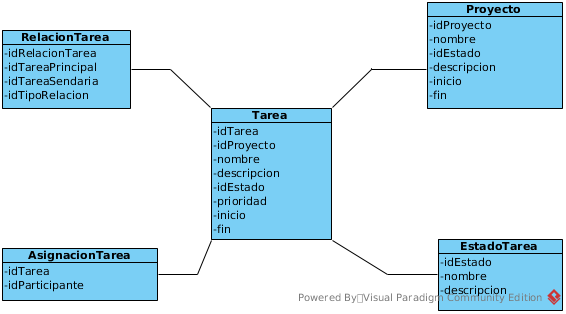
\includegraphics[width=0.8\textwidth]{./images/Modelo_Gestion_Tareas.png}
\caption{Descripción general: Gestión de tareas.} \label{fig:MOD02}
\end{figure}

\newpage

\subsection{Tarea}
\begin{itemize}
	\item \textbf{Nombre} Denominación que se le da a la tarea. Es una palabra corta y este dato es requerido (no se puede omitir). Este atributo debe contener a lo mas 150 caracteres.
	\item \textbf{Descripción} Información de lo que se tratá la tarea. Es un parrafo que describe la tarea, este es un dato opcional. Este atributo debe contener a lo mas 300 caracteres.
	\item \textbf{inicio} Fecha en la cual inicia la tarea. Es una fecha con el formato dd/MMM/yyyy, este es un dato requerido (no se puede omitir).
	\item \textbf{término} Fecha en la cual términa la tarea. Es una fecha con el formato dd/MMM/yyyy, este es un dato requerido (no se puede omitir).
\end{itemize}

\subsection{Asignacion de tarea}
\begin{itemize}
	\item \textbf{Tarea} Tarea a la cual se le asignara un participante.
	\item \textbf{Participante} Participante que se asignara a alguna tarea.
\end{itemize}

\subsection{Estado Tarea}
\begin{itemize}
	\item \textbf{Nombre} Denominación que se le da a estado de la tarea. Es una palabra corta y este dato es requerido. Este atributo puede contener a lo más 25 caracteres
	\item \textbf{Descripción} Descripción sobre el estado de la tarea. Es un parrafo de texto y este dato es obligatorio. Este atributo puede contener a lo más 25 caracteres.
\end{itemize}